\documentclass[12pt]{article}
\usepackage{graphicx}
\usepackage{listings}
\usepackage{subfig}
\usepackage[font=small,labelfont=bf]{caption}
\usepackage{amsmath}

\title{Scholarly Context, Information Divergence, and HTTP link request dynamics:\\
Validating some techniques for characterizing reference rot}
\date{May, 2016}
\author{James Powell, et al}
\pagenumbering{arabic}
\begin{document}
\maketitle
\begin{abstract}
\end{abstract}
\section{Introduction}
Science, like all human endeavors, is embedded in a rich tapestry of interactions that encompass space, time and individuals. To a large degree, scientific progress is reflected in and measured by publications. Yet these publications are themselves embedded in a fragile web. Similarly, legal precedent builds upon itself and decisions intertwine with one another and increasingly with online content, which may or may not be available as time passes. Even the venerable crowd-sourced encyclopedia Wikipedia contains many entries with broken further reading and external links. The word context is often used as shorthand for this organic, supportive network of connections. The scholarly context surrounding a research paper is comprised of the aggregate references that the author(s) uses and explicitly cites in the bibliography of a research paper. An individual researcher's best efforts to organize and reduce disorder in documenting scientific research eventually succumbs to the effects of increasing entropy, because the context is not entirely or likely at all under the control of the researcher, or indeed of anyone else. Items in this fragile context web can change over time, or even disappear forever.

Passive, topically neutral archiving of Web content has been occurring for quite some time, but many objects change too frequently to be adequately preserved, or may not have been archived at all. When one or more archived copies do exist, a reader may access an approximately accurate version corresponding to the original context, at a later date, via technologies such as Memento. Proactive archiving allows the researcher to push a snapshot of a cited reference, as it appeared when cited, into a repository archive from which readers can retrieve it. Other archives were established exclusively to house web at large content, including dark web content, for posterity. Moving forward, robust solutions that combine archiving with link decorations which are HTML attributes have been proposed to allow authors to explicitly indicate cite time and to reference an archived copy while at the same time maintaining a link to the current live cited reference, if it still exists. Many of these solutions have emerged from the Hiberlink [] project which studies reference rot and investigates solutions to it. 

Reference rot encompasses two conditions that affect scholarly context: link rot and content drift. We use a property graph to model the scholarly context for a publication at a given time interval. This yields new variations for the definitions for link rot and content drift which use the language of graphs, but first let's consider why this is an appropriate way to model scholarly context.
\begin{itemize}
\item{The Web is a graph of content objects and HTTP links}
\item{A scholarly paper contains a collection of citations, so the combination of a research paper and its citations constitutes a graph. Citation graphs have been extensively studied, and are often used to evaluate graph metrics in graph theory}
\item{HTTP protocol documentation refers to extended redirect conditions as chains and loops, both of which are also types of graph structures (loops are more commonly referred to as cycles)}
\end{itemize}
\subsection{The characteristics of reference rot for a scholarly context graph are defined as …}
\begin{description}
\item[Link Rot]The edge between the scholarly publication and a given reference has changed. The path may have become longer (e.g. via a redirects which can sometimes result in loops, or cycles, which by definition do not terminate), or the path may lead to a dead end, which is no longer connect to the desired node at all. This is a problem because when a scholarly context path no longer exists, the user is unable to locate the originally cited object. Changes to the path length and structure can also be an ominous sign of problems to come.
\item[Content drift]Properties of the object represented by this node that was originally referenced by the scholarly publication have changed. Sometimes these changes are modest and do not affect the original meaning, but in other cases the object represented by this node may have changed dramatically. This is a problem because the reader may not be able to recognize that this change has occurred.
\end{description}
In our graph model for reference rot, nodes in the scholarly context graph are the content represented by the URI cited for a given Web at large object, and edges are the path to those nodes. HTTP response headers become a source of edges and intermediate nodes in some cases. For example, HTTP redirects can be thought of as resembling blank nodes in RDF graphs, because they lack the definitive characteristics of content nodes (e.g. URLs, textual or binary content), and redirects are not directly addressable Web objects. In this context network, paths grow or break, and node properties drift until sometimes the edge connects to something that the author never intended to reference. The nodes and edges in this graph are  brittle, and subject to change over time. Natural networks which evolve in response to environmental challenges over time in contrast, exhibit characteristics of redundancy and judicious use of hubs. Thus if we can quantify characteristics of reference rot, we might be able to enlist the same strategies evolved in natural networks to improve the situation. Furthermore, this knowledge can inform an evaluation of reference rot solutions suggested to date. These include techniques which archive original content and mint persistent links, or provide temporal (re-)discovery, which seek to preserve or relink the broken portions of the scholarly context graph.  So, while we are not redefining reference rot, thinking about the problem in a graph-oriented manner, as we will show can suggest new ways of thinking about and evaluating the reference rot problem.

This paper presents the results of an investigation into the reference rot problem which monitored the web at large references of a selection of research papers from two archives: arXiv and PLOS. It quantifies the extent of link rot and content drift over a period of 12  - 14 months. We specifically look for indications that  link rot may be an early indicator of content drift and that content drift may in turn be an early indicator for catastrophic link failure.  Thus a primary focus of this research is the relationship between link dynamics and content drift, which differentiates it from previous work which tend to separately consider link dynamics in relation to link rot, and content characteristics as indicators of content drift We also implemented a tool which we used in an effort to better categorize the types of content drift that occurred. This is based on an aggregate representation of the state of research inputs for a given paper.  The tool provides visual cues as to the state of all the cited Web-at-large references for a given paper. Drift characterization was based on two metrics, where possible: a similarity hash for the binary content of a file, and since more than 97\% of the objects cited were HTML documents, we also generated a feature vector representation of an object for each harvest interval and compared this using a common vector comparison metric to the original cited Web-at-large reference. This tool also provided Memento-based links which could be used to quickly inspect the cited content at each harvest interval so as to facilitate categorization of content drift. This tool also suggested a method for calculating an aggregate “drift score” for each paper. 

\begin{figure}[ht!]
  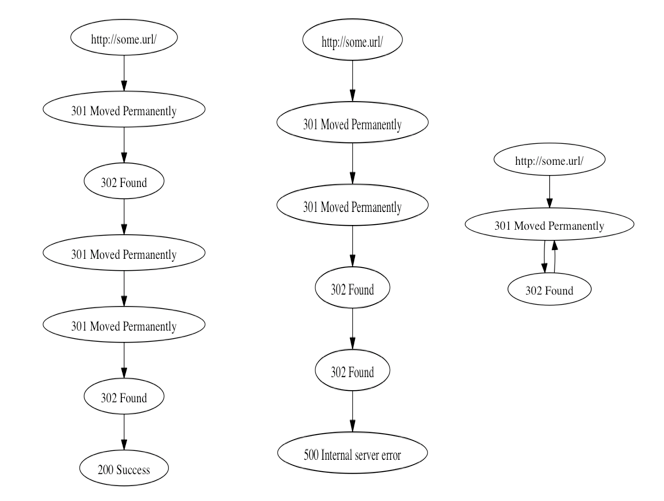
\includegraphics[width=\linewidth,natwidth=610,natheight=642]{figure1.png}
  \caption{HTTP Status chains represented as networks. From left a successful request chain with redirects, an unsuccessful chain with redirects, and a request that results in an endless cycle of redirects}
  \label{fig:statuschains}
\end{figure}

Content drift manifests due to many different challenges and some of these can be content-type specific. With digital images and sound files, content drift can be introduced with the application of a new compression method to the original content.With textual content changes could be introduced through the well-intended efforts of an editor, or an author intent on maintaining the currency of a given resource. Content drift can also manifest as a change in the file type of a cited reference. One example of this would be when a Microsoft Word document is replaced with an un-editable PDF version of the same content. Even though it might be the case that the textual content is identical to the previous version, because the document file format has been changed, the file content can still be said to have drifted because future preservation efforts and access may be affected by this change. 

Quantifying content drift, as others have previously noted [], is a challenge. Optimal quantification of content drift, short of enlisting the original author to retrieve and review references, is only possible if you have an original representation of the referenced Web at large resource at the time it was cited. With binary (e.g. non-textual) files, one of the quickest and most effective ways to detect content changes is to compute a hash representation of the original object and for any subsequent copy, and then compare these hashes. This approach has many applications including detecting song matches in music archiving services and discovering plagiarism (?). The hash similarity approach also works for textual content, but as we will discuss later, there are good reasons to augment this approach with other measures when comparing text documents. 

When an edge in a scholarly context network fails, a reader may see an HTTP error message from a Web server such as 404 indicating the referenced item was not found. Or the server referenced in the URI be unreachable. An edge can be said to have deteriorated when the file has been moved to a new server or a different location which is reachable via one or more redirects. In other words, the path length between the citing and cited reference has increased. Redirects are not necessarily bad, and they are an appropriate way for systems administrators to manage and maintain access to content over time as circumstances necessitate server renames or file reorganization. But a longer path length can portend problems in the future, for example when administrators change or when the reason for a redirect is not documented. When there are more edges there are more opportunities for something to go wrong.

This paper also looks at the HTTP response dynamics in relation to content availability and content drift. To evaluate the implications of content length and status changes in relation to link rot and content drift, we first looked at the trends for content length to change over time, by inspecting the initial content length value for a cited reference, and comparing that to each subsequent content length reported for that reference. Next, we looked at content length changes in relation to similarity changes, to see if content length indicated that there'd also been content drift. Finally, to determine if status chain dynamics implied content drift, we looked at prior interval status chain and end status and compared the content similarity measures for the previous interval with the current interval to see if status changes and longer status chains portend content drift or link rot.
\section{Related Work}
Analyzing the Persistence of Referenced Web Resources with Memento 
Scholarly Context Not Found: One in Five Articles Suffers from Reference Rot
\section{Methodology}
 corpus of papers was identified for arXiv and for PLOS. The content of each paper was then retrieved and stored locally. Next, the content of each paper was parsed to identify all Web-at-large citations. The links within the content were identified and extracted (excluding DOIs), and these became the targets of recurring harvests.  Each URI component of a citations were then used to harvest the original cited reference content. The textual content of the scholarly publication was extracted from the original PDF document and converted to an XML representation. The XML file was then parsed to identify references and their URIs. Next, the content referred to by the cited reference was retrieved, if it still existed. At the same time the cited reference was harvested, all HTTP status headers were also recorded and stored.  These statuses include HTTP response status, redirects, content length, and MIME type. At 30-day intervals, the cited references were again harvested . Thus we accumulated a record of the original scholarly context and a subsequent copy of that context at regular intervals representing both the nodes and edges in that context sub graph.
\begin{center}
 \begin{tabular}{||c|c|c||} 
 \hline
 Corpus & Papers & Distinct cited web at large resources \\ [0.5ex] 
 \hline\hline
 arXiv & 3635 & 12558 \\ 
 \hline
 PLOS & 2060 & 5167 \\
 \hline
 \hline
\end{tabular}
\end{center}
The results of this harvesting constitute two distinct collections of data that tell us something about how the cited references are evolving. The metadata, such as file size and mime type speak directly to aspects of the referenced content. If a PDF file suddenly changed to a JPEG file, then we know there's likely been a significant change even without examining the content. The HTTP status codes tell us if the object, or a redirect surrogate node was returned immediately (200 response), was returned in conjunction with one or more redirect nodes (301, 302, etc), or not found at all (404).

\begin{itemize}
\item Examples of chains that end in success
\begin{enumerate}
\item{301 302 301 301 302 200}
\item{301 301 301 301 301 301 200}
\end{enumerate}

\item Examples of chains that end in failure
\begin{enumerate}
\item{302 301 301 404}
\item{301 301 302 302 500}
\end{enumerate}

\item Examples of cycles / loops (pattern repeats up to the maximum of 50 requests)
\begin{enumerate}
\item{301 302 301 302 301 302 301 302 301 302 301 302 301 302 301 302}
\item{301 301 301 301 301 301 301 301 301 301 301 301 301 301 301 301 }
\end{enumerate}
\end{itemize}

\begin{figure}[ht!]
  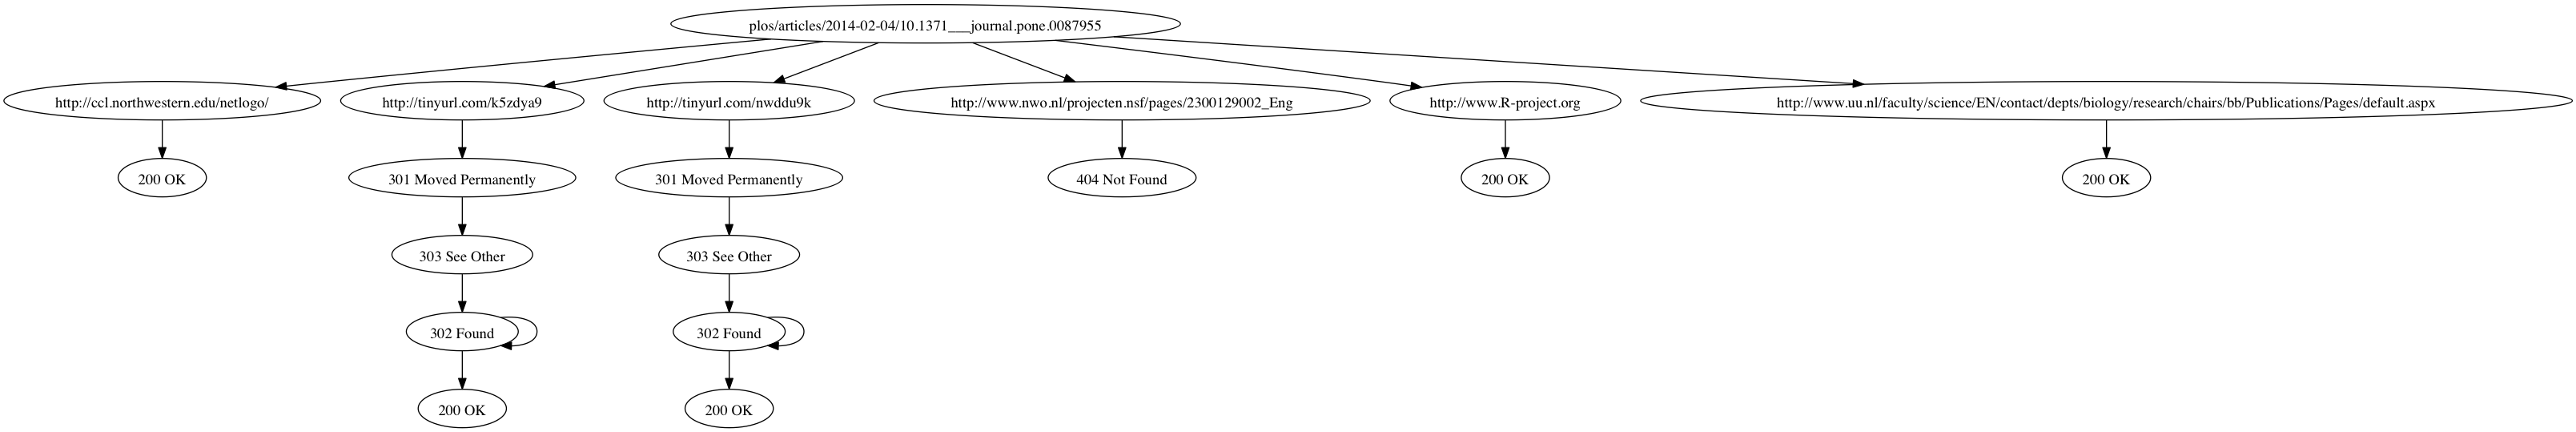
\includegraphics[width=\linewidth,natwidth=610,natheight=642]{figure2_a.png}
  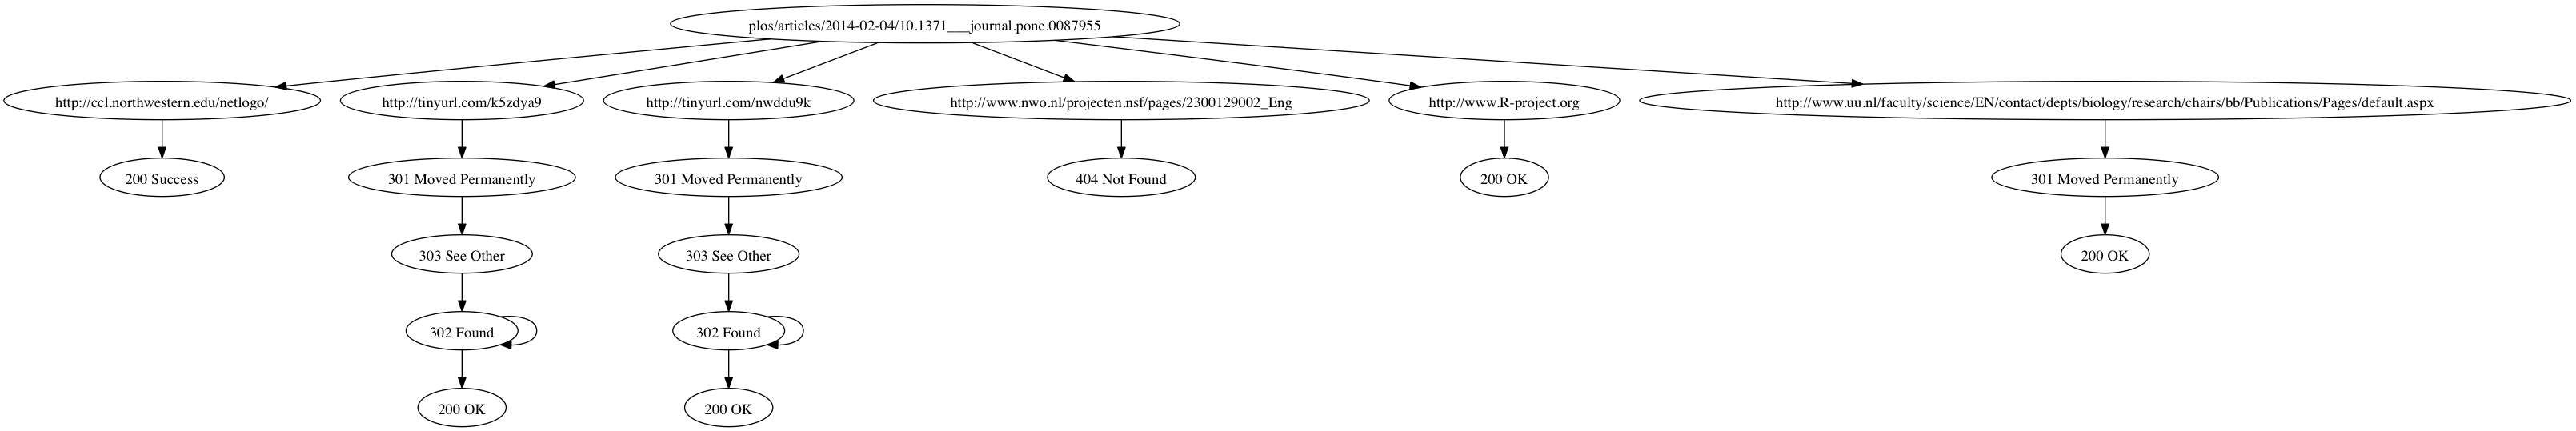
\includegraphics[width=\linewidth,natwidth=610,natheight=642]{figure2_b.png}
  \caption{A scholarly context for a paper at the first harvest interval and at the 14th interval}
  \label{fig:scholcontext}
\end{figure}

Evaluation of the accumulated data included characterization of indicators of link rot (HTTP status responses), analysis of HTTP headers for clues about potential content drift (changes in content length or mime type), and the application of various content representation and comparison techniques (feature vectors, content hashes) to identify and characterize the extent of content drift. Since both HTTP headers and the referenced content was harvested and stored for each interval, it was possible to evaluate changes in a step-wise fashion as well as from the start of the experiment to its completion. 

\begin{lstlisting}[caption=301 Response]
HTTP/1.1 301 Moved Permanently
Date: Thu, 30 Jan 2014 21:20:27 GMT
Server: Apache
Location: http://physics.unm.edu/CQuIC/Qcircuit/
Content-Length: 246
Connection: close
Content-Type: text/html; charset=iso-8859-1
Set-Cookie: Oreo=1968220352.20480.0000; path=/
\end{lstlisting}

\begin{lstlisting}[caption=200 Response]
HTTP/1.1 200 OK
Date: Thu, 30 Jan 2014 21:20:27 GMT
Server: Apache
Last-Modified: Wed, 07 Sep 2011 17:12:32 GMT
ETag: "5d93cb-1340-cb58000"
Accept-Ranges: bytes
Content-Length: 4928
Connection: close
Content-Type: text/html; charset=UTF-8
\end{lstlisting}


Finally, the content of the retrieved reference for each interval provided us with a way to directly compare the content at thirty day intervals. As mentioned earlier, we used a hash as the most basic way of representing and comparing content. After the references were initially harvested, all subsequent copies were compared with the original content, and a similarity score was generated based on the original document's hash as compared to the copy's hash. Later, for textual content, we also generated feature vectors for the original reference and copies, and calculated a normalized percent similar score based on cosine similarity (angle between the original document feature vector and the copy's feature vector). We also use Shannon Entropy and Kullback-Liebler Divergence to characterize content change over time.

\begin{figure}[ht!]
  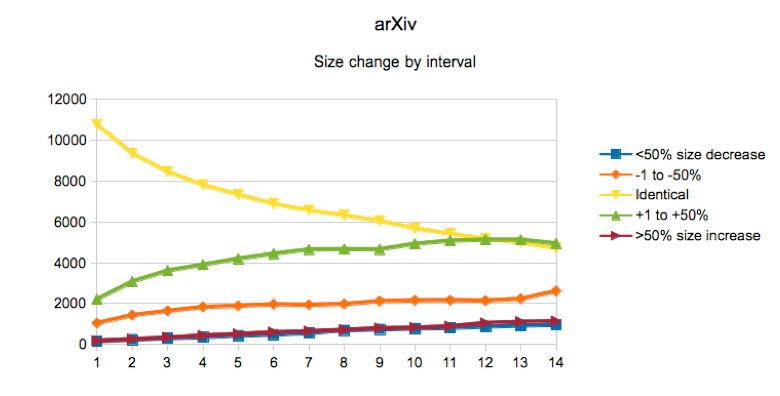
\includegraphics[width=\linewidth,natwidth=610,natheight=642]{figure3.png}
  \caption{Content length change by interval for arXiv cited references}
  \label{fig:arxivclchange}
\end{figure}

Descriptive statistics for arXiv corpus cited references 
\begin{itemize}
\item 3,635 items in corpus
\item 17,158 citations with 14,966 unique Web at large URLs
\item 222,594 instances of these URLs harvested during the experiment period
\item 97.82\% were HTML documents
\item 74.06\% of the cited items changed size
\item 74.5\% of the originally cited items that were available at start were always available
\end{itemize}

\begin{figure}[h!]
  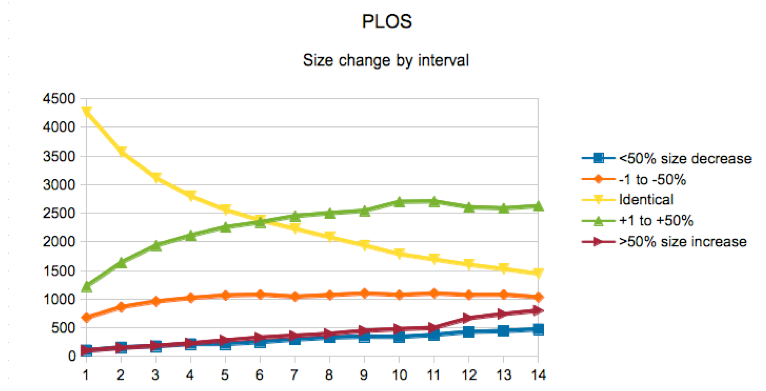
\includegraphics[width=\linewidth,natwidth=610,natheight=642]{figure4.png}
  \caption{Content length change by interval for PLOS cited references}
  \label{fig:plosclchange}
\end{figure}

Descriptive statistics for PLOS corpus cited references
\begin{itemize}
\item 2,060 items in corpus
\item 8,284 citations with 6,549 unique URLs
\item 97,408 instances of these URLs harvested during the experiment period
\item 99.12\% were HTML documents 
\item 80.84\% of cited originals changed size
\item 69\% of originally cited items that were available at start were always available 
\end{itemize}


\begin{figure}[ht!]
  \centering
  \subfloat[Interval 1]{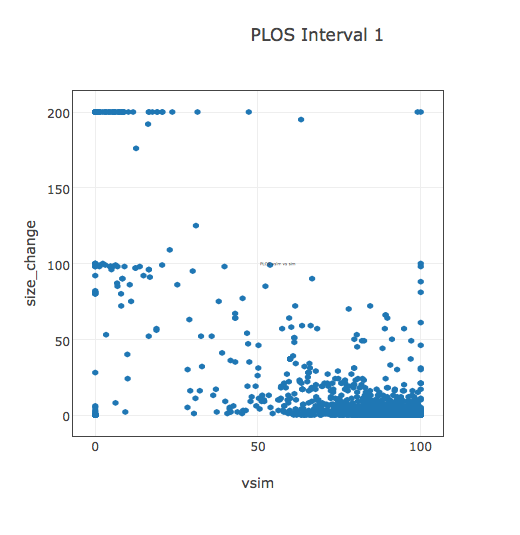
\includegraphics[width=0.4\textwidth]{figure5_a.png}\label{fig:vsimsize1}}
  \hfill
  \subfloat[Interval 14]{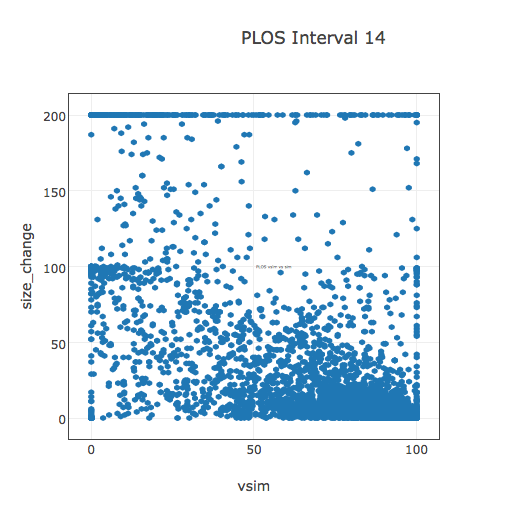
\includegraphics[width=0.4\textwidth]{figure5_b.png}\label{fig:vsimsize2}}
  \caption{Size change verses feature vector similarity, first and last intervals observed, PLOS web at large cited references}
\end{figure}

As with any experiment which depends upon uninterrupted Internet access, there were minor glitches in content harvesting. A scheduled interval harvest occurred during a network outage, resulting in the loss of some data for a portion of the corpus. To compensate for that, all data pertaining to cited references for the affected items were removed from the data set. 

\begin{figure}[ht!]
  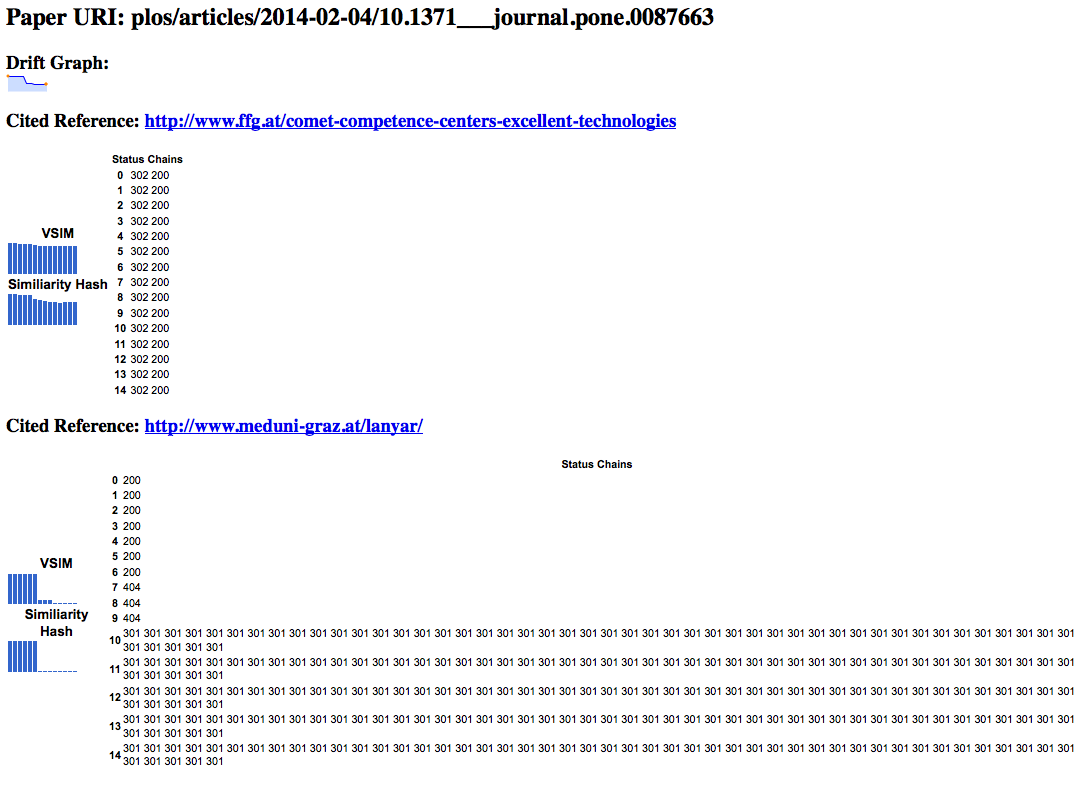
\includegraphics[width=\linewidth,natwidth=610,natheight=642]{figure6.png}
  \caption{Scholarly context inspection interface displaying web at large aggregate content drift and cited reference drift and their respective status chains for experiment duration for one PLOS paper}
  \label{fig:contextinspec}
\end{figure}

By characterizing the metadata (file and HTTP status), and comparing the content over time, we were able to explore a number of questions regarding content drift, some related to link deterioration, and others which characterize the content change over time in different ways.

\begin{itemize}
\item Is size change correlated with content drift?
\item Can content drift result in reduced informational content? How often?
\item Do long chains portend content drift
\item Can soft 404s can be discovered by similarity measures
\item Is content drift usually a gradual rather than sudden phenomena?
\item How soon does the scholarly context of most articles start to exhibit problems? within 3 months?
\item Does content drift tend toward increased entropy?
\end{itemize}

\begin{figure}[ht!]
  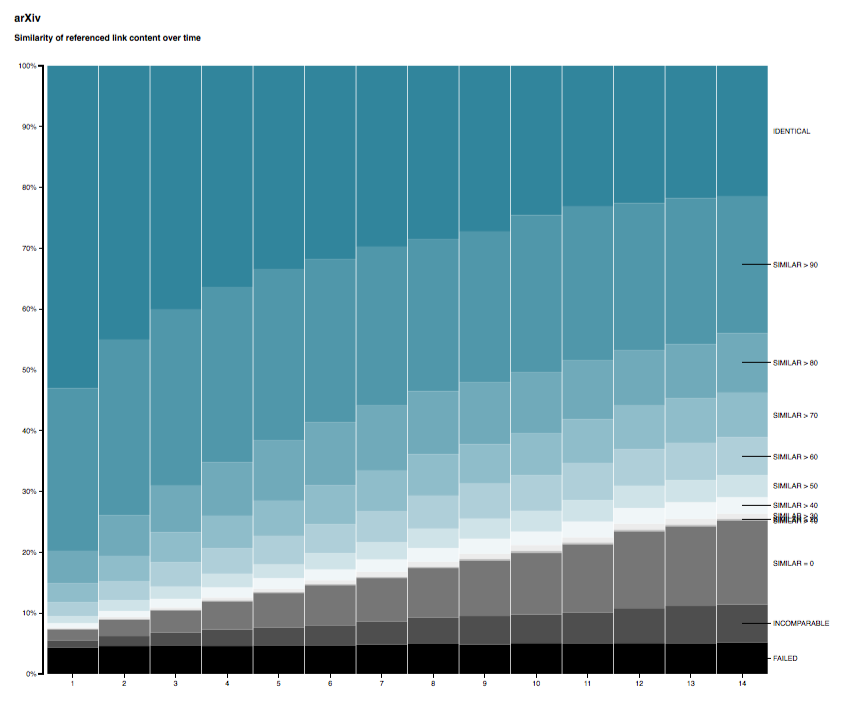
\includegraphics[width=0.65\textwidth]{figure7_a.png}
  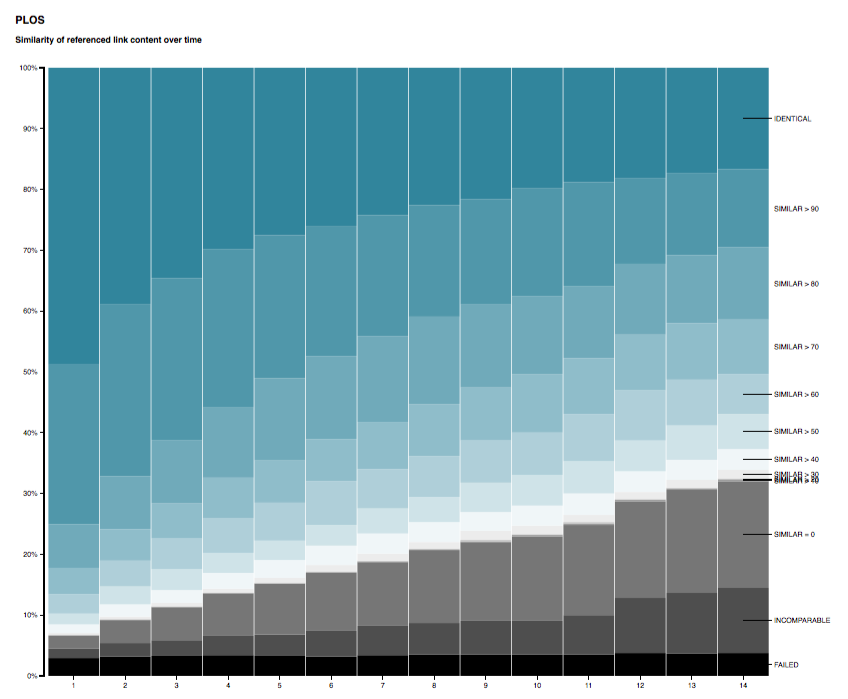
\includegraphics[width=0.65\textwidth]{figure7_b.png}
  \caption{Content drift for arXiv and PLOS cited references over time }
  \label{fig:cdarxivplos}
\end{figure}


\section{Results}
HTTP statuses are perceived as a primary indicator of link rot. When examining the potential for link rot, certain statuses are of particular interest depending on whether they occur at the beginning or end of a potential chain of statuses returned before the object itself is located and returned. If the final HTTP status of a request is a 404 or related status, then the object request failed, the object was not returned, there is no path to the original node, and so link rot is indicated. For other requests, in cases where the first status returned by the Web server was a 3xx status, then there's a potential for link rot, because this indicates that the object has moved. In such cases we follow the path for up to 50 hops, that is 50 HTTP status responses. We found that for PLOS, there was a 34\% increase in 4xx (e.g. 404) statuses for Web-at-large reference. There was also a 28\% increase in 3xx statuses, which indicate that one or more redirects were returned in response to content requests. The percentages for arXiv were lower but still significant: there was a 12\% increase in 4xx statuses and an 11\% increase in 3xx statuses. However, the actual numbers are small. For example, there were typically 300-400 last HTTP responses statuses that were 4xx out of 6367 requests per interval. 

\begin{figure}[ht!]
  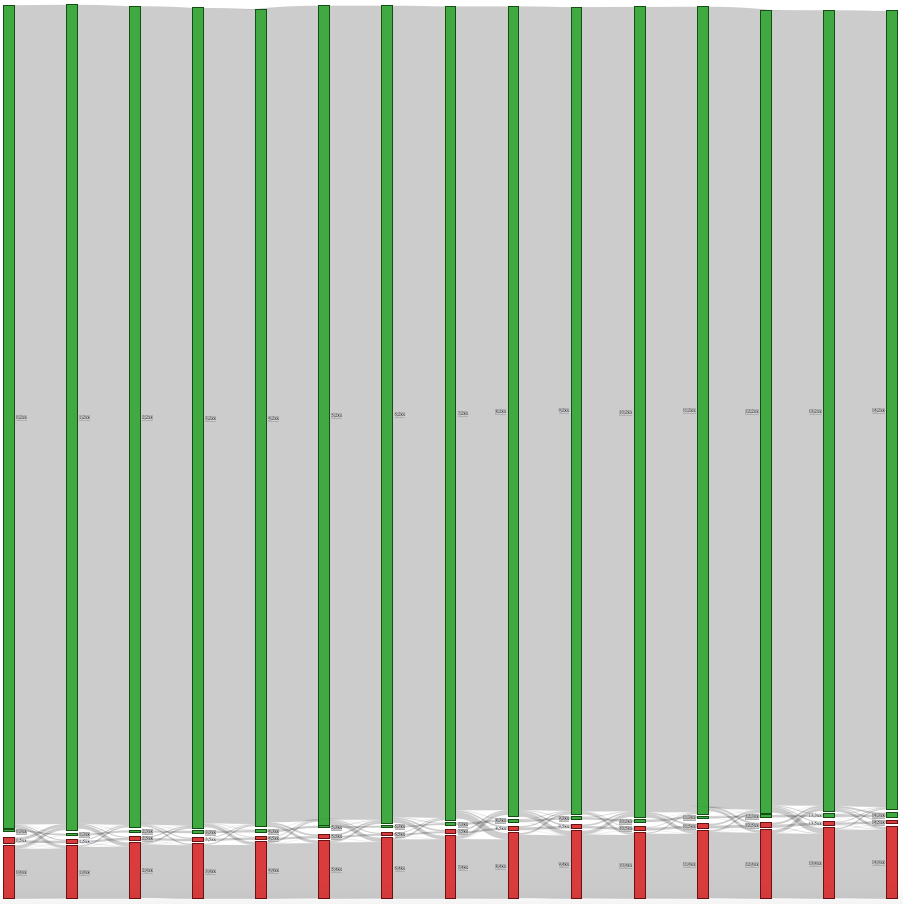
\includegraphics[width=0.85\textwidth]{figure8.png}
  \caption{Link dynamics between intervals – note modest but steady increase in 5xx and 4xx HTTP status responses in red at bottom}
  \label{fig:linkdynam}
\end{figure}
When a status chain results in an object node, HTTP headers contain important clues as to whether content drift may have occurred. The two indicator  statuses are mime type and content length. Mime type changes were almost non existent for the examined resources. However, content length changes were frequent. Content length is compared to the originally retrieved resource, and content length is said to have changed whether the difference for a retrieved copy in a given interval is smaller or larger than the original object. We found that over the course of the experiment, the number of objects that were the same size as the originally retrieved object changed by 66\%  for PLOS and 56\% for arXiv. Furthermore this change occurred rapidly, a surprising number of items had changed size within one interval of the initial harvest (30 days). This suggests that content drift may often occur within weeks after a web at large resource is cited and is generally an ongoing phenomena.

\begin{center}
  \begin{tabular}{|p{3cm}|p{3cm}|p{3cm}|p{3cm}|}
  \hline
  \multicolumn{4}{|c|}{Broken paths} \\
  \hline
  \multicolumn{2}{|c|}{PLOS} & \multicolumn{2}{|c|}{arXiv} \\
  \hline
  none$\rightarrow$4xx & 29 & none$\rightarrow$4xx & 99 \\
  \hline
  none$\rightarrow$5xx & 5 & none$\rightarrow$5xx & 6 \\
  \hline
  2xx$\rightarrow$none & 370 & 2xx$\rightarrow$none & 571 \\
  \hline
  2xx$\rightarrow$4xx & 301 & 2xx$\rightarrow$4xx & 532 \\
  \hline
  2xx$\rightarrow$5xx & 115 & 2xx$\rightarrow$5xx & 388 \\
  \hline
  3xx$\rightarrow$4xx & 4 & 3xx$\rightarrow$4xx & 10 \\
  \hline
  3xx$\rightarrow$5xx & 1 & 3xx$\rightarrow$5xx & 2 \\
  \hline
  3xx$\rightarrow$none & 0 & 3xx$\rightarrow$none & 6 \\
  \hline
  4xx$\rightarrow$none & 36 & 4xx$\rightarrow$none & 105 \\
  \hline
  4xx$\rightarrow$5xx & 15 & 4xx$\rightarrow$5xx & 16 \\
  \hline
  5xx$\rightarrow$none & 8 & 5xx$\rightarrow$none & 7 \\
  \hline
  5xx$\rightarrow$4xx & 21 & 5xx$\rightarrow$4xx & 20 \\
  \hline
  \multicolumn{4}{|c|}{Redirected paths} \\
  \hline
  none$\rightarrow$3xx & 1 & none$\rightarrow$3xx & 2 \\
  \hline
  2xx$\rightarrow$3xx & 41 & 2xx$\rightarrow$3xx & 127 \\
  \hline
  3xx$\rightarrow$2xx & 29 & 3xx$\rightarrow$r23xx & 92 \\
  \hline
  4xx$\rightarrow$3xx & 5 & 4xx$\rightarrow$3xx & 9 \\
  \hline
  5xx$\rightarrow$3xx & 0 & 5xx$\rightarrow$3xx & 3 \\
  \hline
  \multicolumn{4}{|c|}{Repaired? paths} \\
  \hline
  none$\rightarrow$2xx & 343 & none$\rightarrow$2xx & 512 \\
  \hline
  4xx$\rightarrow$2xx & 90 & 4xx$\rightarrow$2xx & 324 \\
  \hline
  5xx$\rightarrow$2xx & 119 & 5xx$\rightarrow$2xx & 368 \\
  \hline

  \end{tabular}
\end{center}


\section{Difference that makes a Difference}
The next question then is has the content actually drifted? We used four techniques to evaluate content  similarity: hash comparisons, feature vector comparisons, Kullback-Leibler Divergence, and human inspection of selected references using the scholarly context inspection interface. Of the four, human inspection is obviously the most precise, but feature vector comparison represented an acceptable compromise in terms of precision and scalability. Although there are many ways to calculate the similarity of two feature vectors, we relied on simple cosine similarity. This has the benefit of normalizing word frequency occurrence, which is desirable if the goal is to determine if the two vectors are essentially about the same thing. Some other measures would impose a penalty for moderate content drift associated with word frequency changes. These measures come closer to answering the question: “is the content the same?” but can yield false negatives if the question is: “is the content essentially still about the same thing?” 

\begin{center}
  Long paths and cycles
  \begin{tabular}{|p{3cm}|p{3cm}|p{3cm}|p{3cm}|}
  \hline
  \multicolumn{2}{|c|}{PLOS} & \multicolumn{2}{|c|}{arXiv} \\
  \hline
  \multicolumn{4}{|c|}{Successful retrieval: 3xx path start, 2xx path end} \\
  \hline
  Length = 3 & 1942 & Length = 3 & 8697 \\
  \hline
  Length = 4 & 1194 & Length = 4 & 1556 \\
  \hline
  Length = 5 & 885 & Length = 5 & 548 \\
  \hline
  Length = 6 & 338 & Length = 6 & 165 \\
  \hline
  Length = 7 & 8 & Length = 7 & 33 \\
  \hline
  & &  Length = 8 & 22 \\
  \hline
  & &  Length = 9 & 30 \\
  \hline
  \multicolumn{4}{|c|}{Failed retrieval: 3xx path start, 4xx path end} \\
  \hline
  Length = 3 & 185 & Length = 3 & 1770 \\
  \hline
  Length = 4 & 79 & Length = 4 & 91 \\
  \hline
  \multicolumn{4}{|c|}{Indeterminate: 3xx path start, 5xx path end} \\
  \hline
  Length = 3 & 5 & Length = 3 & 24 \\
  \hline
  & &  Length = 4 & 4 \\
  \hline
  \multicolumn{4}{|c|}{Cycles} \\
  \hline
  Unterminated 1 node & 41 & Unterminated 1 node & 27 \\
  \hline
  Unterminated 2 node & 5 & Unterminated 2 node & 5 \\
  \hline
  \end{tabular}
\end{center}

Kullback-Leibler Divergence 
Another way to determine whether the content essentially still about the same thing when confronted with two instances of a document that existed at different points in time is to consider the change in the informational content between the two documents. Shannon Information Entropy has long proven to be a reliable metric for evaluating the informational content of a “message.” In his day, a message was an electronic transmission of data, with a temporal component, i.e. contents of the message were ordered in time, and a content component – a distinct collection of symbols that collectively comprised the message. Shannon devised a method for quantifying the informational content of a message using probability. In essence, it calculates the likelihood of a given symbol occurring in the message stream. The technique has found numerous applications in a diverse array of field beyond information science, including biology, chemistry, physics, genetics, and communication where it has been used to quantify the informational content of crystals, molecules and field data, just to name a few examples. The shannon entropy values across original web at large references and copies fell within a narrow band (figure ) which was due primarily to the fact that most of the documents were English language texts. But Shannon Entropy was also a good metric for tracking content change over time and the entropy values closely mirrored other metrics we used. One additional observation of note was that among items that exhibited lower than average entropy (values below the threshold value of 4.0), a manual inspection revealed that the content of at least some of these documents largely consisted of tables of numeric data (recurring symbols). This raises the possibility that it might be possible  to adapt Shannon entropy to reliably identify such tables programmatically in text documents. 

     \[
        H = -{\sum_i} \ {p}_{i} \ log_b \ p_i
     \]

Shannon Entropy can quantify the entropy of a single stream of symbols, but it has inspired and formed the basis of other techniques to quantify the informational divergence between two messages. We used one such technique derived from Shannon Entropy to characterize the informational divergence between copies of cited references over time. Kullback-Leibler Divergence allows one to quantify change in the informational content. We treat the text of the original cited reference as it appeared at the time the citing publication was published as the original message (P). We then use a subsequent copy of that reference harvested at a later point in time as a model (Q) for which divergence is calculated. Using a python implementation of the formula, we generate a list of tokens (i) for each document. Then we iterate through the token list, summing the probability of token i occurring in document P multiplied by the log of the probability of token i occurring in P divided by the probability of token i occurring in Q. As expected, the results show a substantial increase in informational divergence over time (figure 10).

    \[
       D_{KL}({P}\parallel{Q}) = {\sum_i} \ P(i) log \frac{P(i)}{Q(i)}.
    \]

Detecting soft 404 statuses
In some cases, Web server administrators choose to return an HTML document in response to a request for a page that no longer exists. This means that the HTTP response status returned may still be a 200 value, but the page returned has no relation to the originally cited object. We selected a feature vector similarity score of <15\% similar as a threshold for identifying likely phantom 4xx responses, which is probably a rotten link. These totals cover the 14 interval harvest period. Based on this evaluation, up to 4\% of reported PLOS 2xx statuses and  3\% of arXiv 2xx statuses are associated with catastrophic content drift that may in fact represent link rot. KLD scores are also good indicators for catastrophic content drift. In a comparison of KLD scores with HTTP header content length variations over time, the two values exhibited similar patterns of change as the content changed. So content similarity, information divergence, and content length changes, depending on the degree to which the value has changed, are good indicators for phantom 4xx statuses and other forms of catastrophic content drift.  

As discussed earlier the aggregate drift score, which is the mean of the feature vector similarity measures for all cited references for a given paper at a given harvest interval, is an indicator of whether and to what extent the scholarly context of a research paper is affected by content drift. In other words, we summed the feature vector similarity scores for all cited web at large references for a given paper for a given interval, and then divided that value by the number of cited web at large references. It was apparent that many, perhaps most of the corpus was affected by content drift since only 37\% of the PLOS cited web at large references managed to achieve a  feature vector similarity score of 90\% or more over the course of the experiment while 38\% of the arXiv references achieved a similarity score at or above 90\%. Using this data, we then calculated a drift score for the aggregate web at large cited references using their similarity measures per interval. We found that the averaged drift score per interval for the 2060 items in the PLOS corpus never exceeded 60\% and that it fell into the 40\% range by the end of the experiment. This is especially surprising since the average 2xx HTTP status response rate hovered around 90\% for the duration.

By every measure we investigated, content drift increased such that typically less than 20\% of the copies were identical to the original web at large reference by the end of the experiment. This is especially notable given that some measures characterize content drift in significantly different ways than others. For example, size is strictly concerned with the reported content length of the object, while entropy scores a document based on the entropy across all symbols in the textual content stream using Shannon Entropy, yet the number of documents considered identical by these distinct measures was virtually the same. This trend was also evident with vector similarity which one would expect to be good at determining the semantic similarity of two documents, KLD which we used to score a document based on how much it has diverged from the original, and sim hash, which is a coarse grained bit level model of the content stream. Each of these measures were within a few percentage points of one another with respect to the number of items that they identified as being identical to the original cited reference. 

Finally, we evaluated the implications of a long verses a short status chain on the subsequent interval's similarity to the original document. This revealed that long chains consistently resulted in an uptick of variance from the original document by most similarity measures. Only about 40\% of the subsequent interval copies for long chains remained identical to the original item verses more than 50\% for short chains. In other words, a subsequent copy is more likely to have changed if the prior interval request resulted in a longer HTTP response status chain:

\section{Discussion}
The dynamics of paths to web at large resources exhibit churn and degradation just as the availability of such resources and the content they represent tend to decay over time. As the sankey diagram in figure x shows, these paths can change from month to month, and their overall tendency is toward a gradual but definite increase in the percentage of infinite loops, and broken paths that end with internal server errors and 404 not found statuses. However, 2xx response statuses do not necessarily indicate that all is well with a resource. Some 2xx responses mask actual custom 404 response pages while others return content that has drifted significantly from the time it was originally cited. Additionally, one cannot attribute the problem to path degradation as longer paths (containing redirects) only occurred for 4-5\% of of requests, and most of these terminate in 2xx statuses. The only reliable HTTP response status with respect to reference rot is a 4xx, which clearly indicates that the link is rotten. But these account for a fraction  (5-6\%) of the observed statuses. So clearly HTTP statuses alone cannot be used to predict all instances of link rot or content drift. Content length is a more reliable indicator, although the correlation between content length change and feature vector similarity change is not as high as one would expect. One reason for this could be the normalization imposed upon the feature vector when calculating cosine similarity. Word frequency occurrence plays no role in calculating the similarity value, only the presence or absence of a word.  Thus while content length and similarity change over time, they do so at different rates. The drift score reveals that virtually no papers in the corpora studied in this experiment were immune to reference rot. It supports what many others have found in the past – the reference rot problem is common, pervasive and gets worse with the passage of time. The aggregate scholarly context graph around a research paper degraded quickly, and sometimes in ways which would not be obvious to someone reading the paper.  As others have observed, it would be preferable for paths to simply break rather than offer up drifted content. This is why, even though path problems are not severe, solutions that provide more robust paths to the original content are crucial.

Reference rot is a many faceted problem and there is no one size fits all solution. When the scholarly context surrounding a publication is viewed as a network, it is clear that some web at large resources sit at the end of brittle paths and many are in flux and some simply disappear. Robust evolved networks leverage hubs and multiple paths to improve their ability to withstand challenges. The Memento architecture provides a hub-like temporal layer atop content repositories, providing a means to locate best-fit archived resources with respect to a particular time frame. In other words, Memento can often provide multiple paths to the original resource, or to an approximate temporal match. Link decorations inject robustness directly into the scholarly context network by providing a direct path to an archived copy of a web at large resource which was archived by the citing paper author, as well as a path to the current live resource, if it still exists. Unlike regular HTML links, link decorations can provide multiple potential targets for a link. This aspect of link decorations addresses the class of cited references where both the originally cited reference and the most current version may both be of interest (e.g. in the case of a cited reference to a software application). This is associative linking with a temporal component. Thus as with natural networks, these techniques provide robustness in the form of efficient, minimal redundant paths to at risk resources. Indeed some reference rot solutions not only solve the immediate  problem but offer opportunities for scholars to enrich the cited reference experience for readers.

\end{document}
